% !TEX root = ../LinalColloc01.tex

\section{Определение модуля и аргумента. Свойства модуля комплексного числа}
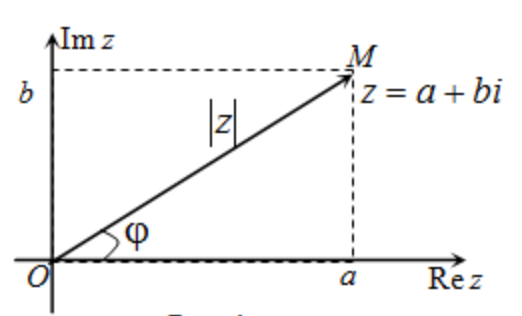
\includegraphics[scale=0.75]{Complex_number_on_plane.png} 
\begin{conj}
    Модулем комплексного числа $z = a + bi$ называется $|z| = \sqrt{a^2 + b^2}$.
\end{conj}
\begin{conj}
    Пусть $z \in \mathbb{C}$, $r = |z|$. Число $\varphi \in \mathbb{R}$ называется аргументом $z$, если 
    \[ z = r(\cos\varphi + i\sin\varphi) \]
\end{conj}
\begin{conj}
    $ z = r(\cos\varphi + i\sin\varphi)$ - тригонометрическая форма комплексного числа.
\end{conj}
\underline{Свойства модуля:}
\begin{enumerate}
    \item $|z| \geqslant 0$ и $|z| = 0 \Leftrightarrow z = 0$
    \item $|\overline{z}| = |z|$
    \item $|z|^2 = z \cdot \overline{z}$
    \begin{proof}
        $z \cdot \overline{z} = (a + bi)(a - bi) = a^2 + b^2 = |z|^2$
    \end{proof}
    \item $|z_1 + z_2| \leqslant |z_1| + |z_2|$
    \begin{proof}
        Будем сравнивать квадраты левой и правой части:
        \begin{gather*}
        |z_1 + z_2|^2 = |(a_1 + a_2) + (b_1 + b_2)i|^2 = (a_1 + a_2)^2 + (b_1 + b_2)^2 = a_1^2 + 2a_1a_2 + a_2^2 + b_1^2 + 2b_1b_2 + b_2^2 \\
        (|z_1| + |z_2|)^2 = a_1^2 + b_1^2 + 2|z_1||z_2|  + a_2^2 + b_2^2 \\
        \Longrightarrow |z_1 + z_2| \leqslant |z_1| + |z_2| \Leftrightarrow a_1a_2 + b_1b_2 \leqslant |z_1||z_2| \\
        \end{gather*}
        Опять возведем левую и правую часть в квадрат:
        \begin{gather*}
            (a_1a_2 + b_1b_2)^2 \leqslant (a_1^2 + b_1^2)(a_2^2 + b_2^2) \\
            2a_1a_2b_1b_2 \leqslant a_1^2b_2^2 + a_2^2b_1^2 \\
            0 \leqslant (a_1b_2 - a_2b_1)^2
        \end{gather*}
    \end{proof}
    \item $|z_1z_2| = |z_1||z_2|$
    \begin{proof}
        Возведем левую и правую часть в квадрат:
        \begin{gather*}
            |z_1z_2|^2 = |(a_1a_2 - b_1b_2) + (a_1b_2 + a_2b_1)i|^2 = (a_1a_2 - b_1b_2)^2 + (a_1b_2 + a_2b_1)^2 = a_1^2a_2^2 + b_1^2b_2^2 + a_1^2b_2^2 + a_2^2b_1^2 \\
            |z_1|^2|z_2|^2 = (a_1^2 + b_1^2)(a_2^2 + b_2^2) = a_1^2a_2^2 + b_1^2b_2^2 + a_1^2b_2^2 + a_2^2b_1^2
        \end{gather*}
    \end{proof}
\end{enumerate}